We compare the performance of 4 memory management strategies 
\begin{description}
\item[\none] -- which does no compaction of the data, this was previously the default in HBase.
\item[\basic] -- which compacts the representation of the index; this is the default in HBase 2.0.
\item[\eager] -- which compacts both the data and index.
\item[\magic] -- which compacts the index or both the data and the index based on the workload.
\end{description}

We compare the strategies by measuring their throughput and latency. In addition we measure the write volume, that is the number of KB written to the file system, and the cumulative gc time of each run.

The results of the following experiments are presented:
(1) demonstrating the insight from different sets of experiments showing that gc overhead is a great throughput predictor,
(2) evaluating different settings of the \basic\ strategy in order to find its optimal configuration,
(3) write-only workload - comparing all 4 strategies,
(4) mixed read-write workload - showing reduction in read latencies of \basic\ and \magic\ strategies with respect to \none.

\paragraph{Experiment setup.}

Our experiments run on 2 clusters with different hardware. 
The first cluster consists of five 12-core Intel Xeon 5 machines with 46GB RAM and 4TB 
SSD storage, interconnected by 1G Ethernet. 
The second cluster consists of five 8-core 
Intel Xeon E5620 servers with 24GB RAM and 1TB magnetic drive. The interconnects  are 1Gbps Ethernet. 
We denote these clusters as the SSD cluster and HDD cluster, respectively.
In both clusters we allocate three nodes to HBase nodes, 1 master and 2 region servers, one to simulate the client whose performance we measure, and one to simulate background traffic
as explained below. Each HBase node runs both an HBase region server or master within 8GB JVM containers and the underlying 
Hadoop File System (HDFS) server . 

The traffic is driven by a client running the popular YCSB benchmark~\cite{Cooper}. 
We run write-only and mixed read-write workload where keys are chosen either from either a zipfian or uniform distribution over 100 millions keys.
In all the experiments we create a table with 4 columns (in a single column family) which is pre-split into 50 regions. 
Each update operation writes 25 Bytes values to all 4 columns of a single key, namely writing 100 Bytes of data.


\paragraph{GC overhead.}

Our experiment show that in write-only workloads gc and throughput have a very high correlation. 
Figure~\ref{fig:gc-throughput-log2} plots the scatter graph of cumulative gc time vs write throughput of several write-only experiments of the system with varying settings in different strategies. It clearly shows that  the lower the gc overhead is, the higher the throughput is.
Specifically, there is a negative linear correlation between their values on a log-log scale.

\begin{figure}[htb]
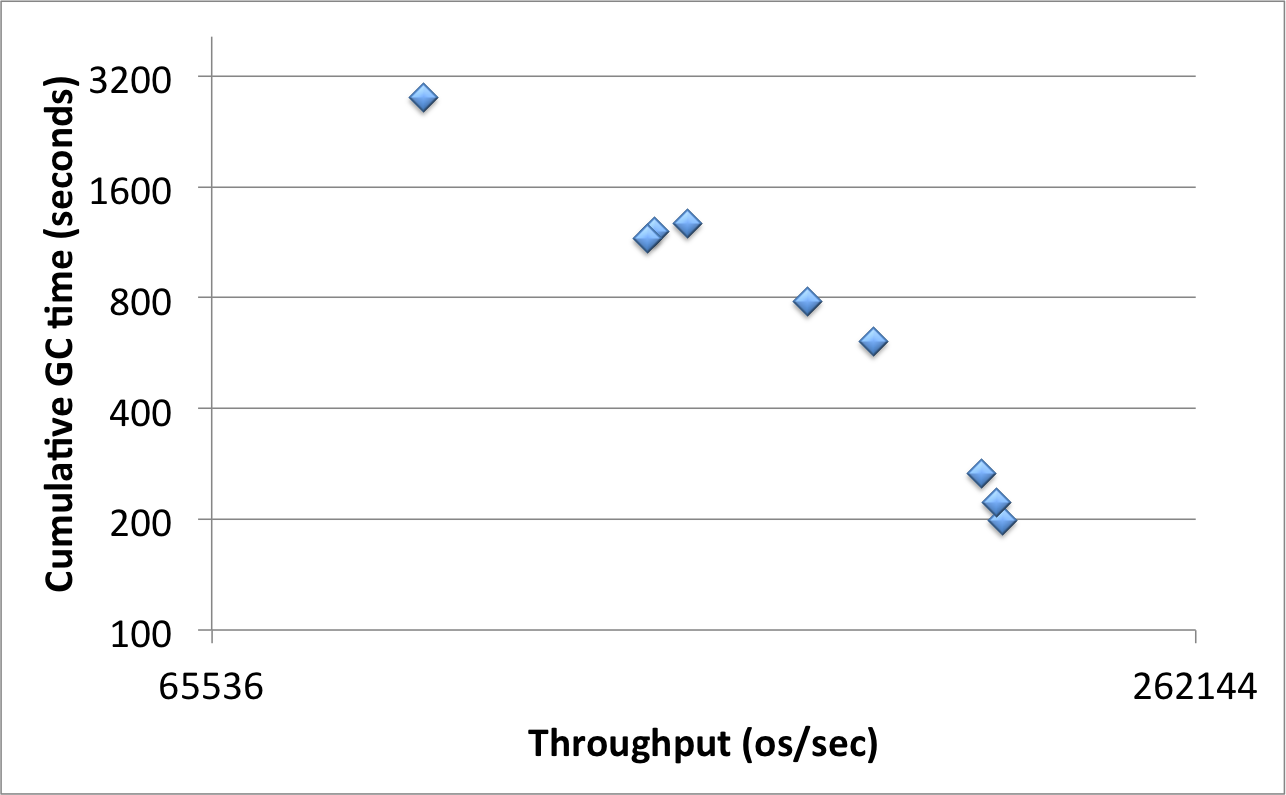
\includegraphics[width=\figw]{Figs/gc-throughput-log2.png}
\caption{{\bf GC-Throughput correlation.} Log-log scale plot of the cumulative gc time vs write throughput in different settings shows negative linear correlation.
}
\label{fig:gc-throughput-log2}
\end{figure}

\paragraph{Parameter exploration.}
One of the main sources for memory management overhead is the skip-list data structure used to index the dynamic fraction of the memory component.
Not only it is bigger in size compared to a flat index it is also fragmented whereas static index is stored in a consecutive block of memory, therefore it incurs smaller overhead in terms of allocation, gc and cache misses.
We evaluate \basic\ strategy with different dynamic fraction sizes. We measure their throughput in write-only workload with zipfian distribution.
An experiment creates an empty pre-split table and then runs 500 million update operations, each writing to all columns. Each such experiment is repeated 5 times. 
The throughput results of all experiments are depicted in 
Figure~\ref{fig:dynamic-fraction}. 
The \none\ strategy has no static portion in the memory component therefore its throughput is added at the point where the dynamic fraction size is equal to 1.0.
Figure~\ref{fig:dynamic-fraction} shows that indeed the store scales as the dynamic fraction size decreases. 

\begin{figure}[htb]
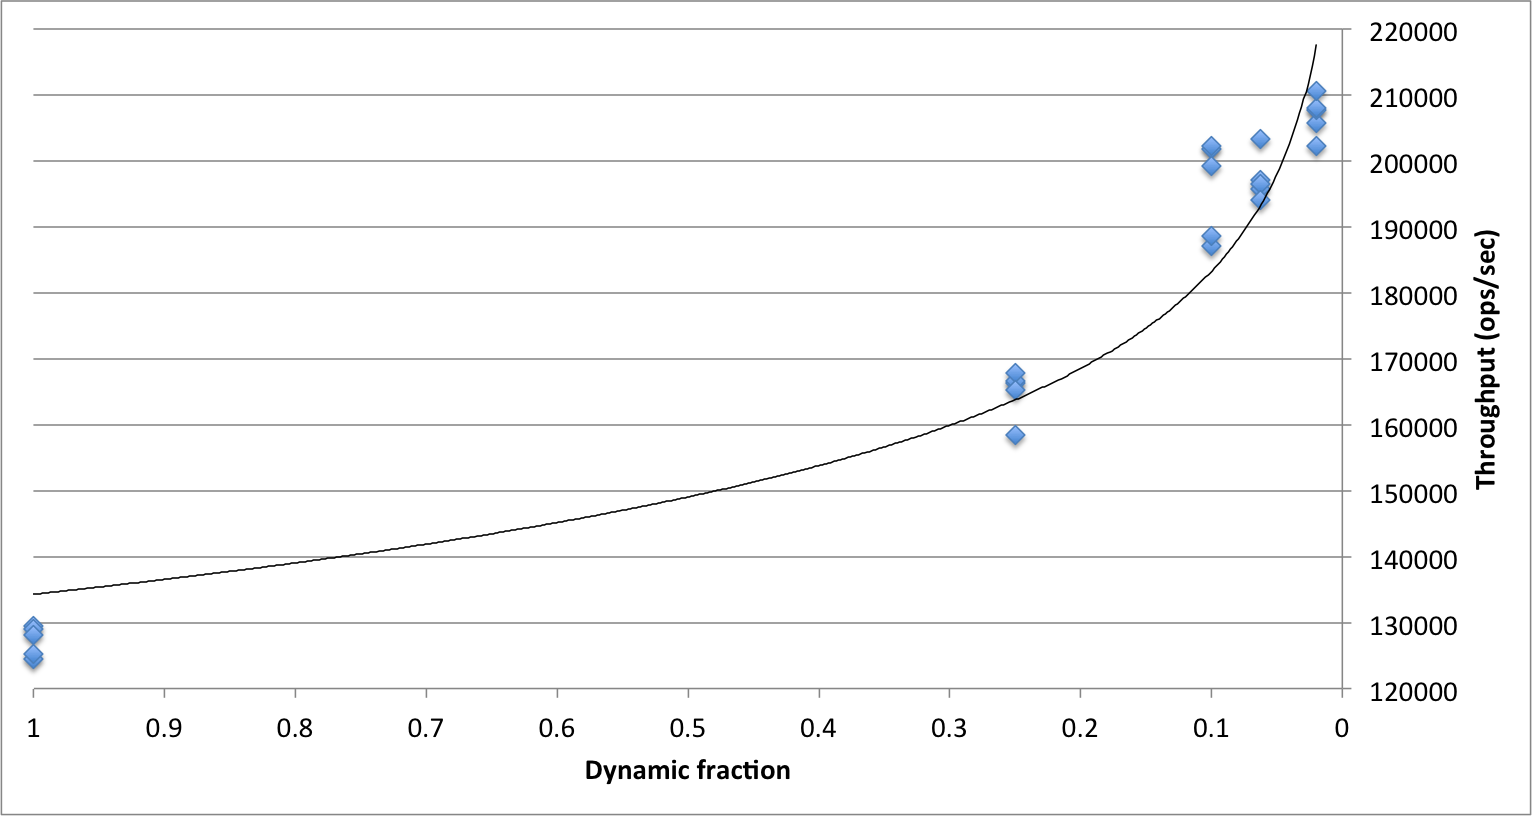
\includegraphics[width=\figw]{Figs/dynamic-fraction.png}
\caption{{\bf Dynamic fraction tuning.} The throughput increases as the dynamic fraction size decreases.
}
\label{fig:dynamic-fraction}
\end{figure}

When the dynamic fraction is fixed to 2\% it is clear that merging it into the much bigger static data over and over again can be inefficient as it creates a new index and dismisses the old one. 
The alternative is to push dynamic segments into the pipeline  several times before they are merged to a single static segment. This helps with creating new index less frequently.
On the flip side, each segment in the pipeline calls for a separate scanner during read operations which can degrade their performance.
Hence, we run the same experiments as explained above, varying the limit for the size of pipeline.
Figure~\ref{fig:pipeline} depicts the throughput results as a function of the pipeline size. Peak throughput is with 4 entries in the pipeline.

\begin{figure}[htb]
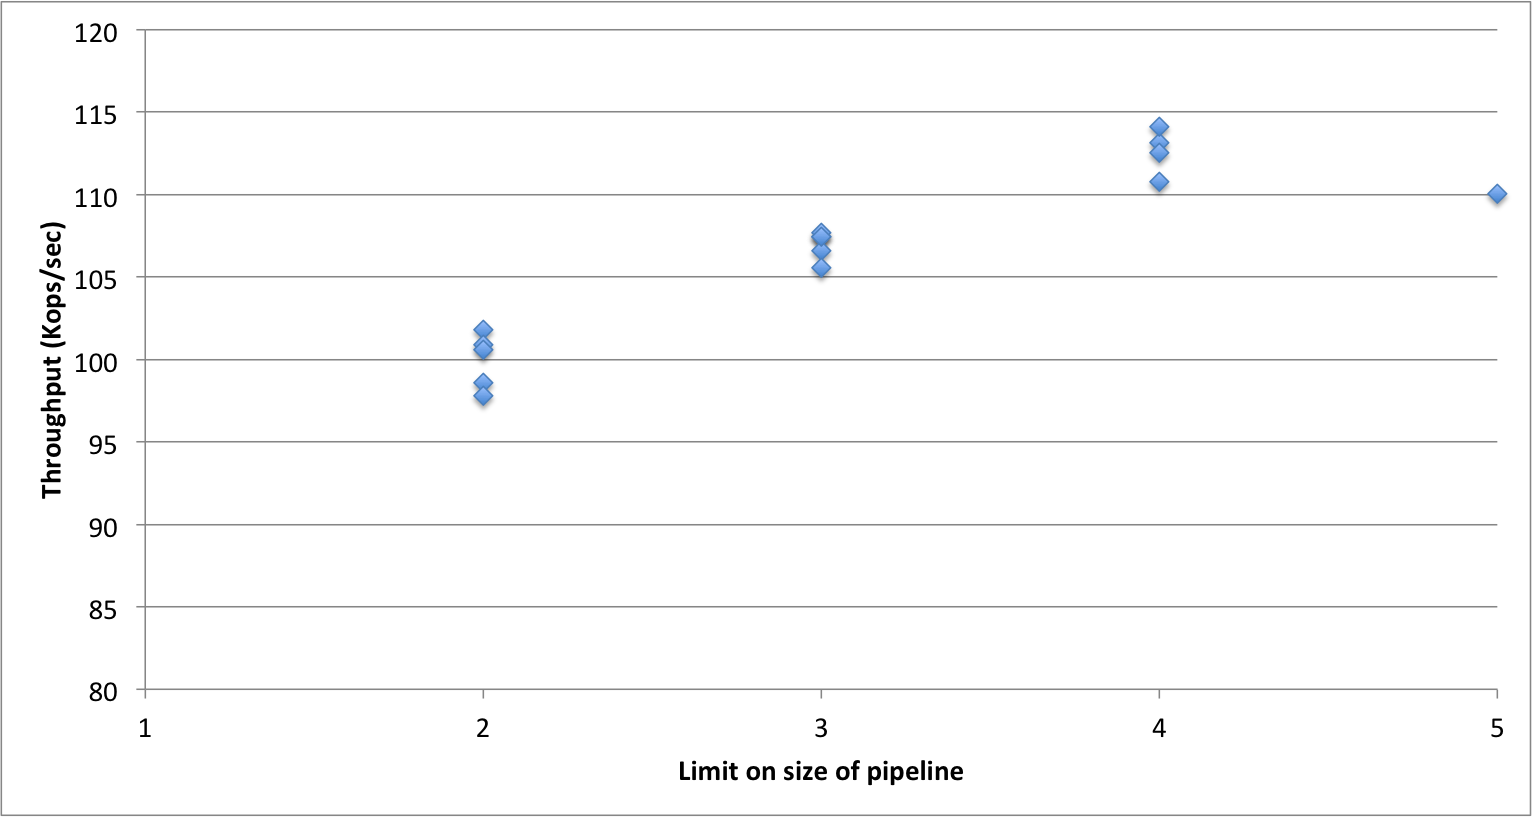
\includegraphics[width=\figw]{Figs/pipeline.png}
\caption{{\bf Pipeline size tuning.} Throughput increases with the size of the pipeline.
}
\label{fig:pipeline}
\end{figure}

\paragraph{Write-only workload.}

\paragraph{Mixed workload.}
